\documentclass[11pt]{article} 
\usepackage[brazil]{babel}
\usepackage[utf8]{inputenc}
\usepackage{boxedminipage}
\usepackage{setspace}
\usepackage{fancyhdr}
\usepackage{latexsym}
\usepackage[pdftex]{graphicx}
\usepackage{float}
\usepackage[hyphens]{url}

\usepackage{multicol}
\usepackage{verbatim}
\usepackage{graphicx}
\usepackage{tabularx}

\pagestyle{empty}

\setlength{\topmargin}{-2.5cm}
\setlength{\textheight}{25.5cm}
\setlength{\oddsidemargin}{-1cm}
\setlength{\evensidemargin}{-1cm}
\setlength{\textwidth}{17cm}
 
\begin{document}

\begin{center}
{\sf {\large Bacharelado em Ciência da Computação}}

{
   \sf {\textbf{MAC0242 - Laboratório de programação}}

Segunda prova -- 12/11/2011
}
\end{center}


\bigskip

%\noindent\begin{minipage}{0.8\textwidth}
\begin{spacing}{2}
\noindent Nome  : \hrulefill

\noindent Assinatura : \hrulefill
\end{spacing}
%\end{minipage} \ \
%\begin{minipage}{0.295\textwidth}

\vspace{1.0cm}
\centering
\begin{spacing}{1.5}
\begin{tabular}{|c|c|c|} \hline
Questão & Valor & Nota \\ \hline
Q1 & 1.5 & \\ \hline
Q2 & 2.0 & \\ \hline
Q3 & 1.5 & \\ \hline
Q4 & 3.0 & \\ \hline
Q5 & 2.0 & \\ \hline
total & 10.0 & \\ \hline
\end{tabular}
\end{spacing}
%\end{minipage}
\vspace{1.0cm}
%\bigskip

\begin{boxedminipage}{\textwidth}
\begin{enumerate}
\item A prova é \textbf{individual} e pode ser feita a lápis.
\item É permitido a consulta a livros, apontamentos ou Internet.
\item Não é necessário apagar rascunhos no caderno de questões.
\end{enumerate}
\end{boxedminipage}

\bigskip

\vspace{2cm}
\begin{flushright}
Boa prova !
\end{flushright}

\newpage

\begin{itemize}
\item[{\bf Q1.(1.5)}]
A questão refere-se às classes abaixo:  
\begin{verbatim}
abstract class Cidadao {
    public abstract String getRG() ;

    public void print() {
        System.out.println("Impressão do cidadão") ;
    }
}


class ZéMané extends Cidadao {
    public String nome = "José Manoel" ;
}


class TestaZé {
    public static void main(String[] args) {
        ZéMané ze = new ZéMané();
        System.out.println("O nome do Zé é: "+ze.nome) ;
    }

}
\end{verbatim}

\begin{itemize}
\item[{\bf Q1a.(0.5)}] Existe um problema relacionado à herança com a classe
  ZéMané. Diga qual é e apresente uma possível correção.
\item[{\bf Q1b.(1.0)}] Quais os possíveis motivos para se utilizar herança?
  Qual é o motivo mais apropriado para descrever a herança a partir de
  classes abstratas e interfaces? Explique como este tipo de herança funciona.
\end{itemize}

% %%%%%%%%%%%%%%%%%%%%%%%%%%%%%%%%%%%%%%%%%%%%%%%%%%%
\hrule
\begin{itemize}
\item[{\bf Q1a.}] O problema relacionado à classe ZéMané é que ela é concreta
mas não implementa o método abstrato getRG() da classe mãe Cidadao, o que é
inválido segundo a herança de objetos. Implementar o método na classe ZéMané
resolve o problema. Uma possível implementação é a seguinte:

\begin{verbatim}
class ZéMané extends Cidadao {
    public String nome = "José Manoel";

    public String getRG(){
        return "123456-X SP";
    }
}
\end{verbatim}

\item[{\bf Q1b.}] Os possíveis motivos para utilizar herança são os de aumentar
a reusabilidade e extensibilidade do código. Através da herança há uma redução
da duplicação de código entre classes semelhantes pois este pode ser
fatorado para uma superclasse e reaproveitado a partir dela. Ainda, o código
fica aberto a incrementos de funcionalidade já que a base está pronta,
precisando ser apenas especializada.

O motivo mais apropriado para descrever a herança a partir de classes abstratas
e interfaces é o de evitar os problemas induzidos através do uso de herança além
de trazer maior flexibilidade. Ao utilizar-se da herança geralmente ocorre uma
violação do encapsulamento entre classes mãe e filha já que muitas vezes a filha
deve conhecer todos os detalhes de implementação da mãe para ser implementada
corretamente. Como consequência, mudar a implementação da mãe pode afetar todas
as filhas. Ainda, a herança pode inviabilizar situações quando um mesmo objeto
precisa assumir diferentes tipos em diferentes momentos, como uma mesma Pessoa
que em um momento é um Professor, em outro Aluno e em outro Funcionário.

O modelo de herança com classes abstratas e interfaces é baseado na composição e 
delegação de métodos. As classes filhas deixam de possuir a relação ``é um'' para
transformá-la em uma relação ``contém um''. Cada classe filha passa a conter uma
referência para a antiga classe mãe e implementam os métodos da mãe delegando
sua execução efetiva para ela. Um exemplo está apresentado abaixo:

    \begin{tabular}{|p{0.5\linewidth}|p{0.5\linewidth}|} \hline
    Herança & Delegação \\ \hline
    \begin{verbatim}
public class Pessoa {
    String nome;
    
    public String obterNome() {
        ...
    } 
}

public class Funcionario
           extends Pessoa {
    private Salario salario;
    
    public Salario obterSalario(){
        ...
    }   
}

public class Aluno
           extends Pessoa {
    private Matricula matricula;
    
    public Matricula obterMatricula(){
        ...
    }   
}
    \end{verbatim}
    &
    \begin{verbatim}
public interface TipoPessoa {
    public String obterNome();
}

public class Pessoa {
    String nome;
    
    public String obterNome() { 
        ...
    } 
}

public class Funcionario
           implements TipoPessoa {
    private Salario salario;
    private Pessoa pesssoa;
    
    public String obterNome(){
        return pessoa.obterNome();
    }
    
    public Salario obterSalario(){ 
        ...
    }
}

public class Aluno 
          implements TipoPessoa {
    private Matricula matricula;
    private Pessoa pesssoa;
    
    public String obterNome(){
        return pessoa.obterNome();
    }
    
    public Matricula obterMatricula(){
        ...
    }
}
    \end{verbatim}
     \\ \hline
    
    \end{tabular}


\end{itemize}
%%%%%%%%%%%%%%%%%%%%%%%%%%%%%%%%%%%%%%%%%%%%%%%%%%%%

\newpage
\item[{\bf Q2.(2.0)}] O sistema ao qual trata esta questão foi retirado da
  primeira fase de um projeto que foi entregue por alunos (veja a figura~\ref{figNum}):

\begin{figure}[htb]
\begin{center}
\includegraphics[scale=0.25]{diagramaFeio3.png}
\end{center}
\caption{Números arbitrariamente grandes.}
\label{figNum}
\end{figure}

\begin{itemize}
\item Na implementação destes alunos, os números inteiros arbitrariamente
compridos foram  representados como listas duplamente ligadas. 
\item A classe ListaLigada é uma lista duplamente ligada. Seus nós são
  elementos da classe NóLista, mostrada no diagrama. 
\item As classes Subtração, Multiplicação e Soma servem para aplicar
  operações às listas ligadas que representam os números. Os métodos
  destas classes recebem como argumentos os nós iniciais das listas
  ligadas sobre as quais deve ser realizada a operação, e retorna o nó
  inicial de uma lista ligada que contém o resultado. 
\item A classe Principal, no projeto em questão, fazia a leitura dos
  arquivos de entrada, construía listas ligadas e aplicava as
  operações a elas. Esta classe depende de todas as demais classes, e
  a relação de dependência foi omitida do diagrama para deixá-lo mais
  limpo. 
\end{itemize}

\begin{itemize}
\item[{\bf Q2a.(0.5)}] Aponte dois defeitos deste projeto. Você deve
  levar em conta princípios como abstração de dados, modularidade e
  encapsulamento, assinaturas dos métodos, etc. 
\item[{\bf Q2b.(1.5)}] Proponha correções para os defeitos que você
  mencionou acima, desenhando um diagrama UML do sistema após a
  correção E o esqueleto das classes do sistema de acordo com sua
  proposta. 
\end{itemize}

% %%%%%%%%%%%%%%%%%%%%%%%%%%%%%%%%%%%%%%%%%%%%%%%%%%%
\hrule
\begin{itemize}
\item[{\bf Q2a.}] Dois defeitos do projeto são a violação do encapsulamento das
classes ListaLigada e NóLista graças ao uso de atributos públicos e a baixa
coesão da classe Principal já que ela é possui múltiplas atribuições como
leitura de dados, construção das listas e aplicação de operações.
  
\item[{\bf Q2b.}] 
{\small
\begin{verbatim}
public class NumeroGrande {
    private ListaLigada<Integer> num;

    public NumeroGrande(String numero) {
        construirLista(numero);
    }

    private void construirLista(String numero) { ... }
    public NumeroGrande somar(NumeroGrande x) { ... }
    public NumeroGrande subtrair(NumeroGrande x) { ... }
    public NumeroGrande multiplicar(NumeroGrande x) { ... }
}

public class InterfaceUsuario {
    public void lerDados() { ... }
    public void exibirResultado(NumeroGrande num) { ... }
}

public class Principal {
    private InterfaceUsuario iu;
    public Principal(){ ... }
    public void invocarOperacoes() { ... }
}

public class ListaLigada<T> {
    class NóLista<T> {
        private T conteúdo;
        private NóLista<T> próximo;
        private NóLista<T> anterior;

        public NóLista(T conteúdo) { ... }
        public T getConteúdo() { ... }
        public void setConteúdo(T conteúdo) { ... }
        public NóLista<T> getPróximo() { ... }
        public void setPróximo(NóLista<T> próximo) { ... }
        public NóLista<T> getAnterior() { ... }
        public void setAnterior(NóLista<T> anterior) { ... }
    }

    private NóLista<T> primeiro;
    public ListaLigada() { ... }
    public void inserir(T elemento) { ... }
    public T obter(int posicao) { ... }
    public void remover(int posicao) { ... }
}

\end{verbatim}
}
%\usepackage{graphics} is needed for \includegraphics
\begin{figure}[htp]
\begin{center}
  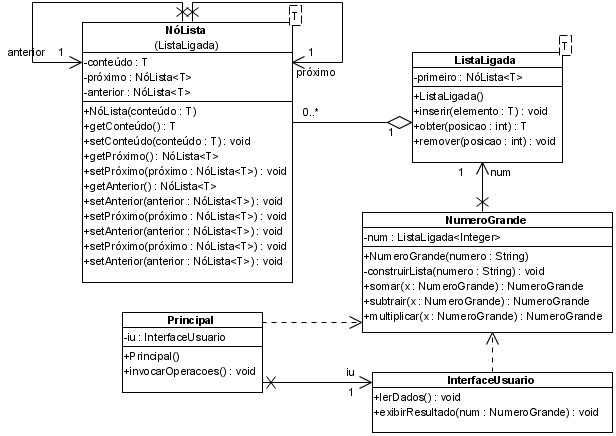
\includegraphics[width=15cm]{recursos/NumerosGrandes.png}
  \caption[Números arbitrariamente grandes - modificado]
  {Números arbitrariamente grandes - modificado}
  \label{numeros-modificado}
\end{center}
\end{figure}

\end{itemize}
%%%%%%%%%%%%%%%%%%%%%%%%%%%%%%%%%%%%%%%%%%%%%%%%%%%%

\newpage
\item[{\bf Q3.(1.5)}]
Modele a seguinte aplicação usando a técnica dos substântivos e verbos
e os cartões CRC (especifique três cenários e desenhe os cartões na
sua prova). 

\textbf{O José desenvolve e instala sistemas de monitoramento (para
  segurança) que consistem de zonas, sensores e uma estação
  centralizada de monitoramento (veja figura~\ref{fig}). Uma zona é
  uma coleção de sensores, tipicamente localizados dentro de uma sala,
  andar, linha de montagem ou prédio. Um sensor é um dispositivo de
  aquisição de dados que mede uma dada variável de sistema e provê um
  sinal de saída para outros dispositivos/sistemas lerem. Por exemplo,
  diferentes tipos de sensores podem detectar temperatura, pressão,
  nível de fumaça, ou movimento. }

\begin{figure}[htb]
\begin{center}
\includegraphics[scale=0.6]{ProvaPOO}
\end{center}
\caption{Sistema de monitoramento do José}
\label{fig}
\end{figure}

\hrule
\begin{description}
  \item[Cenário 1] Usuário deseja verificar a situação de uma determinada
  zona. Desenvolvimento: (i) Usuário informa número da zona que deseja verificar. (ii)
  Estação de monitoramento verifica os sinais de cada um dos sensores da zona.
  (iii) Estação de monitoramento exibe o estado atual de cada um dos sensores da
  zona.
  \item[Cenário 2] Sensor detecta nível anormal na sua variável.
  Desenvolvimento: (i) Sensor detecta nível anormal. (ii) Sensor envia sinal
  para a estação de monitoramento. (iii) Estação de monitoramento processa o
  sinal recebido e notifica a atividade anormal informando qual zona e qual
  sensor a acionou.
  \item[Cenário 3] Nível da variável monitorada pelo sensor retorna ao normal.
  Desenvolvimento: (i) Nível, que estava anormal, retorna aos padrões normais.
  (ii) Sensor desativa sinal para a estação de monitoramento. (iii) A estação de
  monitoramento notifica qual sensor retornou à normalidade.
\end{description}

Cartões CRC:

\begin{tabularx}{\textwidth}{|X|X|}
  \hline
  \multicolumn{2}{|c|}{Classe: Estação de Monitoramento} \\
  \hline
  Responsabilidades & Colaboradores \\ \hline
  Armazena as zonas & Zona \\
  Recebe sinais dos sensores & Sensor \\
  Exibe estado atual de uma zona & Coleção \\
  \hline
\end{tabularx}

\begin{tabularx}{\textwidth}{|X|X|}
  \hline
  \multicolumn{2}{|c|}{Classe: Zona} \\
  \hline
  Responsabilidades & Colaboradores \\ \hline
  Armazena os sensores sob sua responsabilidade & Sensor \\
  Fornece o estado atual dos sensores sob sua responsabilidade & Coleção \\
  \hline
\end{tabularx}

\begin{tabularx}{\textwidth}{|X|X|}
  \hline
  \multicolumn{2}{|c|}{Classe: Sensor} \\
  \hline
  Responsabilidades & Colaboradores \\ \hline
  Verifica nível de uma variável (Temperatura, pressão, movimento, fumaça) &  \\
  Envia sinal para dispositivos quando inicia ou cessa uma atividade anormal  & \\
  \hline
\end{tabularx}

\begin{tabularx}{\textwidth}{|X|X|}
  \hline
  \multicolumn{2}{|c|}{Classe: Coleção} \\
  \hline
  Responsabilidades & Colaboradores \\ \hline & \\ \hline
\end{tabularx}

\newpage
\item[{\bf Q4.(3.0)}] Responda às questões conceituais abaixo. 
\begin{itemize}
\item[{\bf Q4a.(1.0)}] Explique o que são "inner classes", qual a razão de usá-las e dë um exemplo.
\item[{\bf Q4b.(1.0)}] Quais são as principais diferenças entre C\# e Java? Dë um exemplo de código 
de uma das diferenças citadas.  
\item[{\bf Q4c.(1.0)}] Explique como funciona o tratamento de exceções em Java. Por que não se deve 
usar no caso do código abaixo?
\end{itemize}
\begin{verbatim}
...
try {
        for (i=0, i < N, i++) 
            a[i++].f() ;
    } 
catch(ArrayIndexOutOfBoundsException e) {
     ...
}
\end{verbatim}

\hrule
\begin{itemize}
  \item[{\bf Q4a.}] 
  Em Java há o conceito de ``Nested class'', uma classe definida dentro de uma
  outra classe. Inner classes são nested classes que tem acesso aos
  atributos e métodos (Privados inclusive) do objeto que as contém, mesmo os
  privados. Inner classes também podem ser chamadas de Nested classes não
  estáticas. \cite{oracle:nested-classes}
  
  Segundo \cite{carlos:classes-internas} podemos perceber a utilidade das inner
  classes quando há uma relação íntima entre a classe interna e a externa. Isso
  permite evitar a necessidade de adicionar uma nova classe ao projeto que será
  utilizada apenas em um contexto bastante específico. Ainda, 
  \cite{oracle:nested-classes} complementa afirmando que há um aumento do
  encapsulamento já que não há mais a necessidade de prover acesso externo a
  atributos que seriam privados uma vez que a inner class pode acessá-los
  diretamente. Além disso, há um aumento da legibilidade e capacidade de
  manutenção do código já que blocos maiores de código são quebrados em classes
  menores.
  
  Exemplo adaptado de \cite{tony:inner-classes}:
  \begin{verbatim}
public class InterfaceUsuario extends JFrame {
    //Inner class
    class TratadorBotao implements ActionListener {
        public void actionPerformed(ActionEvent e) {
            ...
        }
    }

    private void montaGUI() {
        JButton botao = new JButton();
        botao.addActionListener(new TratadorBotao());
    }
}
  \end{verbatim}
  \item[{\bf Q4b.}] 
    A lista de diferenças entre Java e C\# foi adaptada de 
    \cite{jon:differences-csharp-java}: 
    \begin{itemize}
    \item Java roda em quase qualquer plataforma através da JRE, C\# é uma
    linguagem de propriedade da Microsoft e depende de esforços externos
    (Projeto Mono) para rodar em outras plataformas;
    \item C\# não possui exceções checked;
    \item Java não possui sobrecarga de operadores;
    \item C\# não possui inner classes, apenas nested classes estáticas; 
    \item Java não possui properties como parte da linguagem, apenas uma
    convenção de métodos get/set/is;
    \item Java não possui structs
    \end{itemize}
    
    Exemplo de código retirado de \cite{frank:java-csharp-comparison} para o
    fato de Java não possuir properties:
    
    \begin{tabular}{|p{0.5\linewidth}|p{0.5\linewidth}|} \hline
    Java & C\# \\ \hline
    \begin{verbatim}
private int mSize;

public int getSize() { return mSize; }
public void setSize(int value) {
  if (value < 0)
    mSize = 0;
  else
    mSize = value;
}


int s = shoe.getSize();
shoe.setSize(s+1);
    \end{verbatim}
    &
    \begin{verbatim}
private int mSize;

public int Size {
  get { return mSize; }
  set {
    if (value < 0)
      mSize = 0;
    else
      mSize = value;
  }
}

shoe.Size++; 
    \end{verbatim}
     \\ \hline
    
    \end{tabular}

    \item[{\bf Q4c.}] O sistema de exceções do Java funciona da seguinte
    maneira: quando uma exceção é lançada (throws), a JVM entra em estado de
    alerta e vai ver se o método atual toma alguma precaução ao tentar executar
    esse trecho de código. Caso o método não esteja tratando esse
    problema, a JVM pára a execução dele anormalmente, sem esperar ele terminar,
    e volta um stackframe na pilha de execução, onde será feita nova
    verificação. O processo se repete até que ela encontre algum método que
    trate o erro (catch). Caso não haja nenhum tratador a Thread corrente morre.
    \cite{caelum:apostila}
    
    Não se deve utilizar tratamento de exceções no caso do código apresentado
    pois se \texttt{N} $\leq$ \texttt{a.length} o try-catch seria inócuo já que
    \texttt{i} $<$ \texttt{N} impede que haja um acesso fora dos limites do
    array. Já no caso de \texttt{N} $>$ \texttt{a.length} o correto seria
    alterar o funcionamento do programa para evitar a possibilidade de um acesso
    inválido ao array, tornando desnecessário o uso do bloco try-catch.
\end{itemize}

\newpage

\item[{\bf Q5.(2.0)}] Resolva a questão 5 da segunda lista de exercícios (que está no paca, 
em exercícios preparatórios para a prova).

  \hrule
  \begin{itemize}
    \item[{\bf Q5a.}]
    A ideia principal é tornar o ato de ser informado de algum
    acontecimento um processo assíncrono, ou seja, evitar a necessidade de
    verificar periodicamente (polling) o estado atual de um programa.

    Num programa baseado em eventos, em geral temos um objeto que é o gerador
    dos eventos, e outros objetos que se registram junto a ele, interessados
    naquele evento.

    \item[{\bf Q5b.}]
    Código retirado das notas de aula:
\begin{verbatim}
import javax.swing.*;
import java.awt.*;
import java.awt.event.*;
 class Janela extends JFrame {
   JButton botao = new JButton();

   class EscutaBotao implements ActionListener {
     public void actionPerformed(ActionEvent a){
       System.out.println("Botão apertado");
     }
   }

   public Janela() {
     EscutaBotao eb = new EscutaBotao();
     botao.addActionListener(eb);
     try {
       jbInit();
     } catch (Exception e) {
       e.printStackTrace();
     }
   }

   //Métodos jbInit() e main() não são alterados

 }
\end{verbatim}
    \item[{\bf Q5c.}] O diagrama do código modificado encontra-se abaixo: 
\begin{figure}[htp]
\begin{center}
  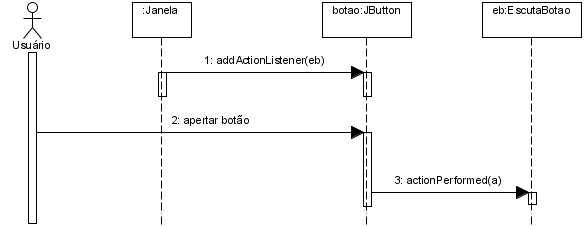
\includegraphics[width=15cm]{recursos/Botao.png}
  \caption[Diagrama de sequências do clique de um botão]
  {Diagrama de sequências do clique de um botão}
  \label{diagrama-botao}
\end{center}
\end{figure}
  \end{itemize}
\end{itemize}

\newpage
\bibliographystyle{abnt-alf}
\bibliography{bibliografia}

\end{document}